\documentclass{llncs}
\usepackage[T1]{fontenc}
\usepackage{lmodern}
\usepackage{color}
\usepackage{amssymb}
\usepackage{amsmath}
\usepackage{galois}
\usepackage{bussproofs}
\usepackage{tikz}
\usetikzlibrary{shapes,arrows,matrix}
\usepackage{url}

\title{Multi-trace Concolic Execution Framework}

\author{Kyel Ok \and Joonwon Choi \and Chanwoo Chung}

\institute{
  \email{\{kyelok, joonwonc, cwchung\}@mit.edu}
}

\begin{document}
\maketitle
%% \begin{abstract}
%%   ABSTRACT
%% \end{abstract}

\section{Introduction}

Concolic execution is a powerful tool to automatically detect bugs
that are difficult to encounter in a normal workflow of an
application. Since rarely used parts of an application is often less
tested, an adversary could exploit bugs in such places by carefully
formulating the inputs to the application. Concolic execution provides
an automated way of preventing such attacks by testing many branches
of the system workflow and catching bugs that are rarely encountered
otherwise.

While standard concolic execution is great for single-user
applications, it is difficult to achieve high code coverage when
testing multi-user applications due to non-determinism introduced. In
a single-user application, the state of an application, i.e., the path
conditions, is only dependent on the inputs of the single user; by
changing the inputs of the user, concolic execution can cover all the
path conditions possible. However, for a multi-user application, the
state of an application is a function of all of the users sharing the
same resources. Thus, without observing the other users, concolic
execution performed on a single user would result in a
non-deterministic behavior.

An example of a non-deterministic behavior observed on a multi-client
application would be when a client tries to register a new user on a
web-based application. If the application was a single-client
application, i.e., only accepts one connection at all times, and if it
reset its database before each concolic execution run, registering the
same user would always work deterministically. However, if there was
even one other client having unobservable interactions with the
server, registering the same user may fail if that client registers
the user beforehand.

Non-deterministic behavior in multi-client applications is an artifact
of unobservability of the entire system. Since a computer is a
deterministic machine, there is no true randomness or non-determinism
in its applications. There are only seemingly non-deterministic
results that are caused by the lack of the ability to quantize all of
the factors of an event. For example, in the scenario for user
registration discussed earlier, if the concolic execution system knew
all the inputs of the other clients it could deterministically
conclude if registering a user would fail or not. In other words, if a
concolic execution system could precisely observe all the interactions
of all the users, it could deterministically define the current state.

Based on the notion of non-determinism being the direct result of
unobservability, we propose a multi-trace concolic execution framework
that can achieve multi-user observability. We propose to have a
high-level process that determines the number of clients interacting
with an application, inputs each client can use, and the timing
difference between the actions of the clients. The path conditions for
the high-level process would expand to include the actions of all the
users and therefore be able to observe the actions of each user.

\section{Multi-trace concolic execution framework}

\subsection{Base framework}

Multi-trace concolic execution we propose starts several parallel
concolic execution client threads that interact with a server. The
idea is that by having each thread represent a single client
interacting with the server, we can simultaneously assign and control
all the clients sharing the same resources.

% TODO: reference in Lab 3
We systematically expand the inputs to a multi-client application
using four growing variables. First, a list of possible concrete
values for any single client is congregated when they are discovered
from attempting to branch in new ways as done in Lab 3. Then, using
such inputs, we form all possible permutations of the inputs that can
be assigned across the client threads. Once each of the unique
permutation has been tested, we increase the number of the processes,
and form a new permutation of the input set for the bigger number of
processes. Lastly, we try different start times of the client threads
for the exact same inputs to capture the full state of an
application. Since clients interacting with a server may produce
different results depending on the order and the timing of commands
executed, including the time variable is beneficial. Finally, this
exponential and infinite growth of the input space is continuously
exploited to explore the states of a multi-client application until
the number of parallel processes reaches a user-defined maximum.

% TODO: [maybe have a flow-diagram or pseudo-code for the 5 loops?]

\subsection{Heuristics for a speed boost}

\subsubsection{Removing the time offset}

The first heuristic we use to speed up the multi-trace concolic
execution system is removing the time difference variable and
executing all the client threads in parallel. We apply our prior
knowledge that most multi-client bugs are caused by a tight race
condition between clients. Thus, it is most likely to reveal a bug
when multiple clients execute commands simultaneously. We confirm this
theory by manually adjusting the time offset between client threads
and verifying the number of bugs the multi-trace concolic execution
system finds.

As seen in Fig. \ref{fig:error}, the results are non-deterministic as
the same offset between clients may or may not produce bugs. We
suspect that the non-determinism is caused by the lack of control over
precise timing between the threads, i.e., the best we can do is
\texttt{sleep()} on an OS that is not real-time, and the lack of
observability of the CPU scheduler that services all the parallel
threads in a linear fashion.

\begin{figure}
  \begin{center}
    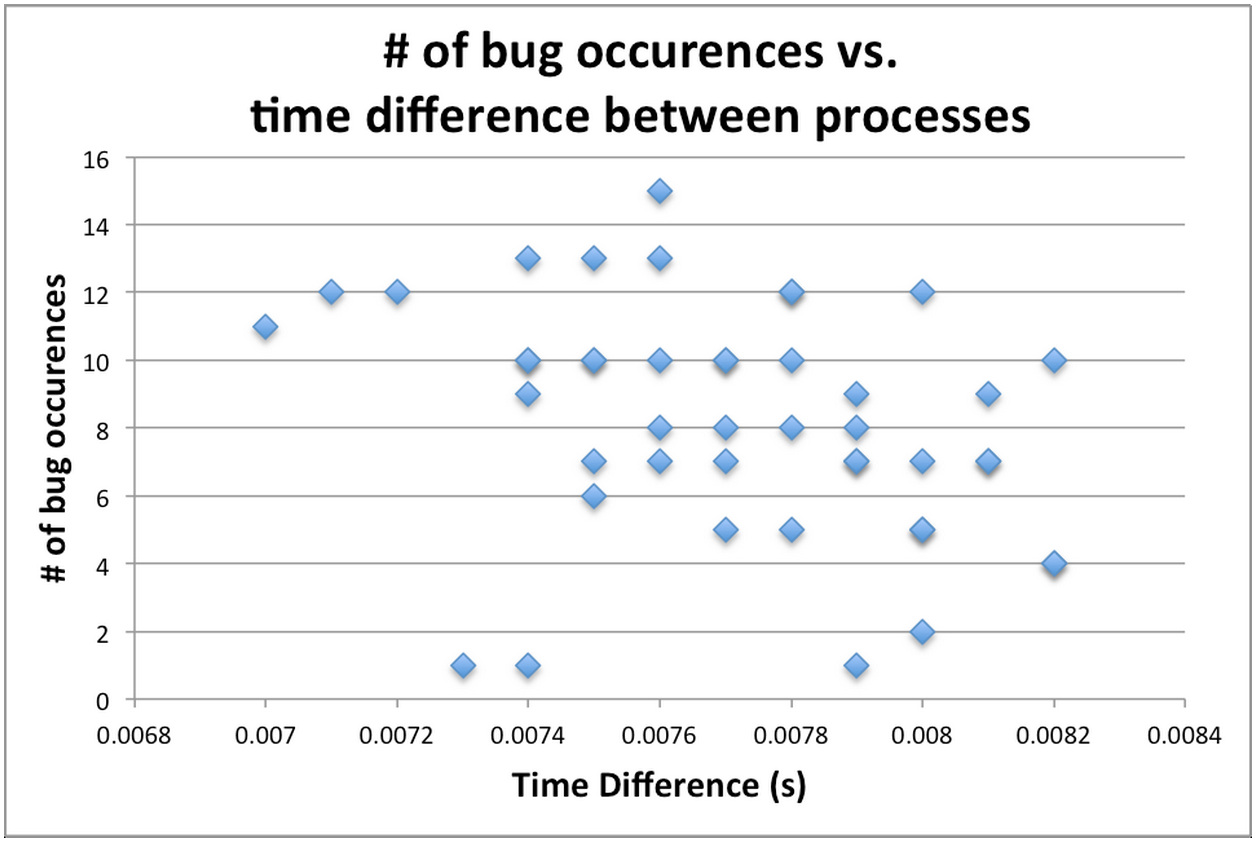
\includegraphics[width=0.9\textwidth]{graph.png}
  \end{center}
  \caption{Bug occurences and time difference}
  \label{fig:error}
\end{figure}

\subsubsection{Constraining the concrete input values}

Another heuristic we can apply is to limit the possible input values,
i.e. the concrete values a client can use, to the ones that are more
likely to cause a multi-client bug. Since we have prior knowledge that
multi-client bugs are mostly caused by invoking shared resources, we
can limit the inputs to those that include a path to sharing
resources. In our experiments, this limitation results in a large
speed boost while still being able to reveal the bugs found without
it.

\section{Experiments}

We have run our multi-trace concolic execution system on zoobar
application to automatically detect possible multi-client bugs that
were missed in the standard single-trace concolic execution done in
Lab 3.

We have found three new bugs in the zoobar application. The bugs are
as extreme as crashing the web browser to having zoobars lost.

\subsection{Timing tests}

We have compared the time taken for multi-trace concolic execution
with and without the heuristics discussed earlier. Table
\ref{fig:speed} shows the results where the heuristics can result in
up to a 1.2 times speed boost. The maximum number of processes was
limited to two for this run.

\begin{figure}
  \begin{center}
    \begin{tabular}{l|c|c}
      \hline
      & normal & with heuristic \\
      \hline
      Bug 1 & 45 seconds & 4 seconds \\
      Bug 2 & 37 seconds & 28 seconds \\
      Bug 3 & 101 seconds & 82 seconds \\
      \hline
    \end{tabular}
  \end{center}
  \caption{Speed boost by heuristic}
  \label{fig:speed}
\end{figure}

% TODO: Experiment table

\subsection{Attack scripts}

We have developed attack scripts to exploit the bugs found using our
multi-trace concolic execution framework.

\section{Conclusions}

We have developed multi-trace concolic execution to find multi-client
bugs in web applications that allow several users to interact with
shared resources. We used the developed concolic execution framework
to uncover three new bugs in the zoobar applications, and have
developed attack scripts to exploit the automatically found bugs.


\end{document}
